\chapter{Az alkalmazás működése}

\section{Authentikáció}

A felhasználók magukat egy email-jelszó párossal tudják azonosítani, melyet regisztrációkor adhatnak meg.

A regisztráció kezelésénék két dologra kellett figyelmet fordítanom: egy email cím csak egyszer szerepelhessen
az adatbázisban, valamint a jelszót megfelelő módon tároljuk az adatbázisban.

Az első kritériumra megoldásként szolgál az adatbázisban az email mező egyedivé tétele, valamint a regisztráció során
a megadott emailcím ellenőrzése.

A jelszó biztonságos tárolása érdekében azt regisztráció során hash-elve mentem el az adatbázisba, erre az \lstinline|argon2| könyvtárat
használtam fel.

\subsection{Megvalósítás}

A session kezeléshez a \lstinline|passport| könyvtárat és cookie alapú megoldást használtam. Ennek során a felhasználót a böngészőben
tárolt cookie információ azonosítja, amit backenden ellenőrzi tudunk.

A frontenden történő ellenőrzéshez egy hook-ot készítettem, mellyel ellenőrzhető, hogy a felhasználó be van-e jelentkezve.

\begin{lstlisting}[caption=Authentikáció hook]
export function useUser() {
  const { data, mutate } = useSWR<{ user: User }>("/api/user", fetcher)
  const loading = !data
  const user = data?.user
  return [user, { mutate, loading }] as const
}
\end{lstlisting}

\section{Authorizáció}

Az alkalmazás megfelelő használata érdekében szükséges volt bizonyos funkciók elérésének szűkítésére. Ehhez a role-based access control
megoldást választottam, mely alapján a felhasználókat különböző kategórákba tudjuk besorolni, majd ezeknek a kategóriáknak adunk jogosultságokat.

Ennek megfelelően három jogosultság-kategóriát hoztam létre: \lstinline|BASIC|, \lstinline|ADMIN| és \lstinline|EDITOR|.

A \lstinline|BASIC| felhasználók képesek foglalást leadni és a sajátjaikhoz megjegyzést fűzni, valamint a hozzájuk tartozó foglalásokat listázni.

Az \lstinline|EDITOR| jogosultsággal rendelkezők ezen felül képesek az egyes foglalások állapotát állítani, valamint bármyely foglaláshoz
megjegyzést fűzni.

Az \lstinline|ADMIN| joggal rendelkezők a fentieken kívül képesek könyvek és kategóriák hozzáadására, törlésére és szerkesztésére.

\subsection{Megvalósítás}

A kódbázison belül a frontenden és backendes is szükséges elleőrizni a megfelelő jogosultságokat.

A backenden ehhez létrehoztam egy middleware-t, amely a már bejelentkezett emberek jogosultságát ellenőrzi.
\begin{lstlisting}[caption=Authorizáció middleware]
const requireRole = (...roles: userrole[]) => {
  return (req: NextApiRequest, res: NextApiResponse, next: NextHandler) => {
    if (roles.some(it => it === req.user.role)) {
      return next()
    } else {
      return res.status(401).json({ message: "Nincs megfelelő jogosultságod" })
    }
  }
}
\end{lstlisting}

A frontenden történő validáció esetén két forgatókönyv lehetséges: egy teljes oldal vagy az oldalon belül bizonyos komponensek
elrejtése a felhasználó elől.

Az előbbi kezelésére létrehoztam egy React hook-ot, amivel az oldalak megjelenítését tudjuk kontrollálni.

\begin{lstlisting}[caption=Authorizációs hook és használata]
// src/lib/hooks.tsx
export function useRequireRoles(roles: userrole[] = []) {
  const [user] = useUser()

  return roles.some((it) => it === user?.role)
}

// src/pages/admin/index.tsx
const hasAccess = useRequireRoles([userrole.ADMIN, userrole.EDITOR])
if (!hasAccess) {
  return <ErrorPage statusCode={401} message="Nincs megfelelő jogosultságod!" />
}
\end{lstlisting}

Az oldalon belüli bizonyos tartalmak elrejtésére készítettem egy komponenst, ami a tartalmát a felhasználó jogosultsági szintjének
megfelelően jeleníti csak meg.

\begin{lstlisting}[caption=Authorizáció komponens és használata]
// src/components/HasRole.tsx
export default function HasRole({ roles, children }: Props) {
  const [user] = useUser()
  const hasRole = roles.some((it) => it === user?.role)

  return <>{hasRole && children}</>
}

// src/components/Navbar.tsx
<HasRole roles={[userrole.ADMIN, userrole.EDITOR]}>
  <NextLink href="/admin">
    <Link>Admin</Link>
  </NextLink>
</HasRole>
\end{lstlisting}

A fenti módszerek alkalmazásásval egy robosztus jogosultság-kezelő megoldást sikerült implementálnom a szoftverbe.

\section{Könyvek listázása}

A kezdőoldalon az elérhető könyveket tudjuk listázni egy rácsszerkezetben.
Itt látható a könyvöz kapcsolt borítókép, a könyv címe, szerzője és kategóriái.

\begin{figure}[!ht]
  \centering
  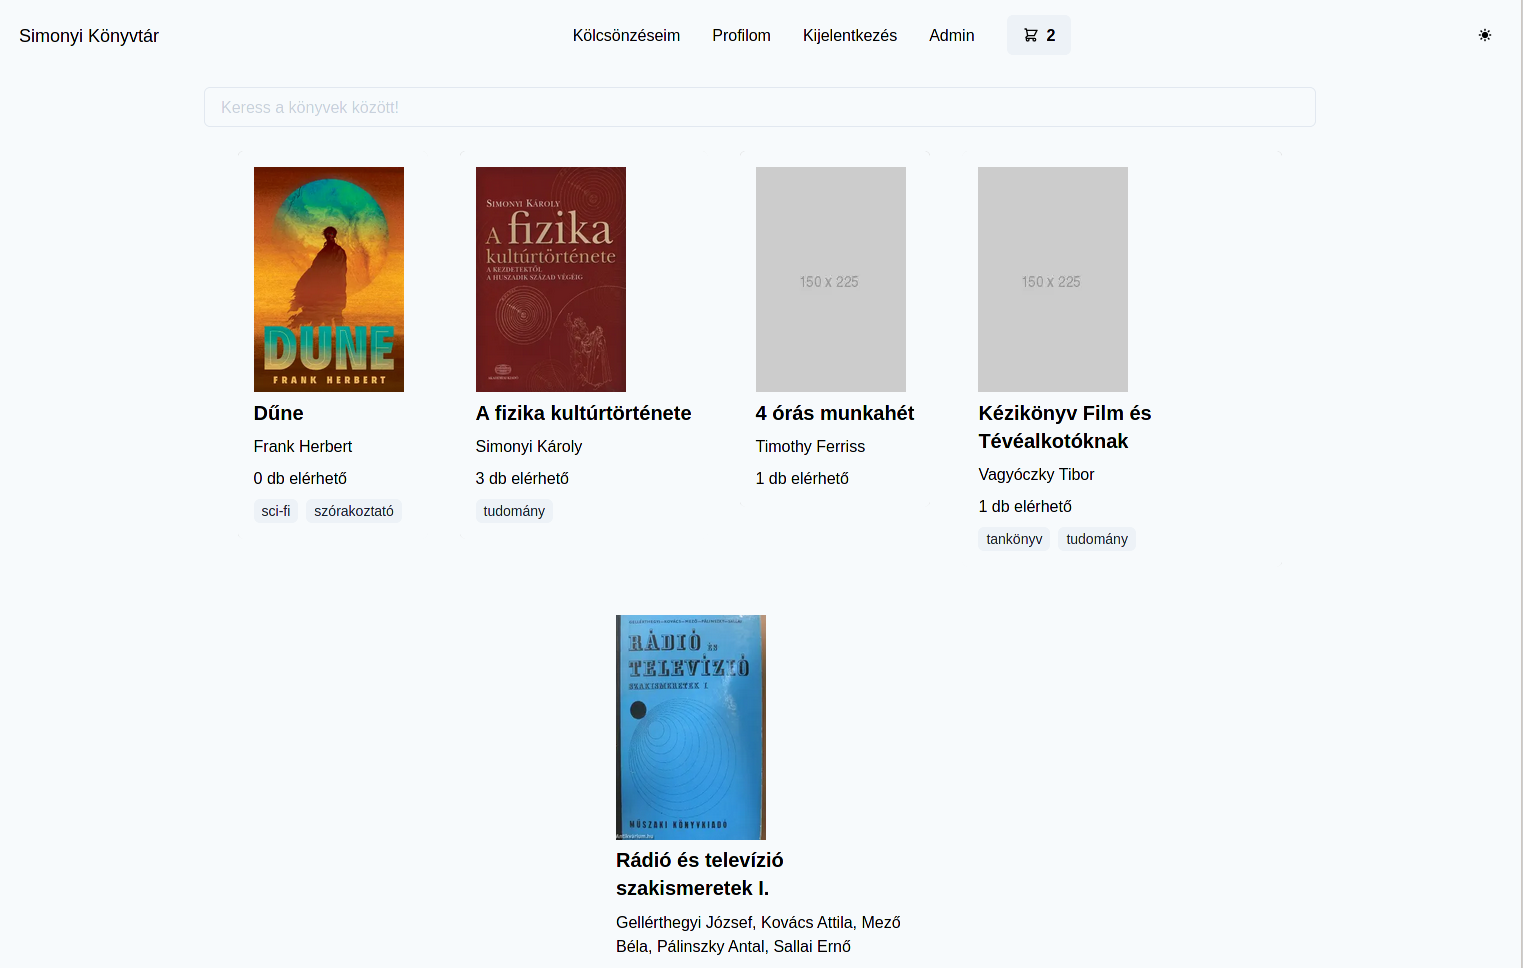
\includegraphics[width=150mm, keepaspectratio]{figures/index.png}
  \caption{Az alkalmazás kezdőlapja}
  \label{fig:IndexPage}
\end{figure}

\subsection{Részletes nézet}

A főoldalon egy könyvre kattintva megkapjuk annak részletes nézetét. Itt láthatjuk az összes hozzá tartozó információt, valamint
lehetőségünk van a könyv kosárba helyezésére (feltéve, hogy van belőle elérhető példány).

\begin{figure}[!ht]
  \centering
  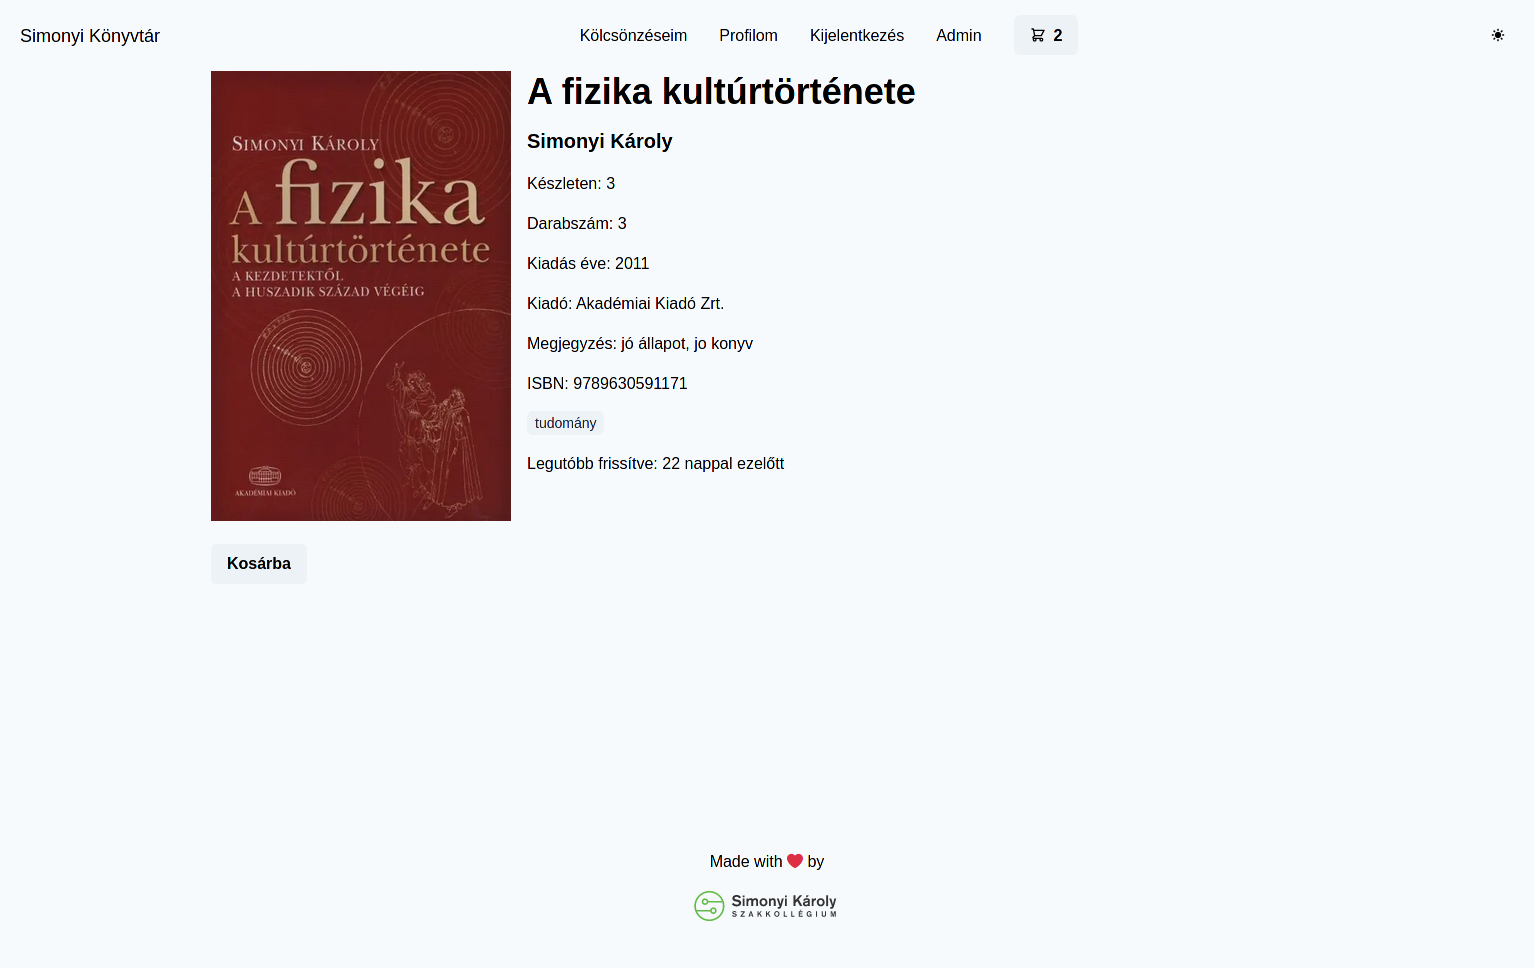
\includegraphics[width=100mm, keepaspectratio]{figures/book-detail-view.png}
  \caption{Könyv részletes nézete}
  \label{fig:BookDetailView}
\end{figure}

\subsection{Keresés a könyvek között}

A főoldalon tudunk a meglévő könyvek közötti kulcsszavas keresésre. Ezt a PostgreSQL Full Text Search funkciójával implementáltam.

Ehhez szükséges volt létrehozni az indexeléshez szükséges oszlopot a \lstinline|Book| táblán, ami alapján az adatbázismotor a kersést
el tudja végezni.

\begin{lstlisting}[caption=A kereséshez szükséges SQL utasítások]
ALTER TABLE "Book"
ADD COLUMN document tsvector;
update "Book"
set document = to_tsvector(title || ' ' || author || ' ' || publisher || '' || notes);

ALTER TABLE "Book"
ADD COLUMN document_with_idx tsvector;
update "Book"
set document_with_idx = to_tsvector(title || ' ' || coalesce(author, '') || ' ' || coalesce(publisher, '') || '' || coalesce(notes, ''));
CREATE INDEX document_idx
ON "Book"
USING GIN(document_with_idx);

ALTER TABLE "Book"
  ADD COLUMN document_with_weights tsvector;
update "Book"
set document_with_weights = setweight(to_tsvector(title), 'A') ||
  setweight(to_tsvector(coalesce(author, '')), 'B') ||
  setweight(to_tsvector(coalesce(publisher, '')), 'C') ||
  setweight(to_tsvector(coalesce(notes, '')), 'D');
CREATE INDEX document_weights_idx
  ON "Book"
  USING GIN (document_with_weights);

CREATE FUNCTION book_tsvector_trigger() RETURNS trigger AS $$
begin
  new.document :=
  setweight(to_tsvector('english', coalesce(new.title, '')), 'A')
  || setweight(to_tsvector('english', coalesce(new.author, '')), 'B')
  || setweight(to_tsvector('english', coalesce(new.publisher, '')), 'C')
  || setweight(to_tsvector('english', coalesce(new.notes, '')), 'D');
  return new;
end
$$ LANGUAGE plpgsql;

CREATE TRIGGER tsvectorupdate BEFORE INSERT OR UPDATE
    ON "Book" FOR EACH ROW EXECUTE PROCEDURE book_tsvector_trigger();

\end{lstlisting}

A keresés implementálásához szükséges volt még egy egyedi lekérdezés írása, ugyanis a Prisma jelenleg nem támogatja a \lstinline|tsvector|
alapú keresést. Ehhez az alábbi megoldást használtam a backenden.

\begin{lstlisting}[caption=Könyvek közti keresés megvalósítása]
const sql = escape(`
select id, title, author, "stockCount", "updatedAt", image
from "Book"
where document_with_idx @@ plainto_tsquery('%s')
order by ts_rank(document_with_idx, plainto_tsquery('%s')) desc;`, term)
const books = await db.$queryRaw(sql)
\end{lstlisting}

Alapesetben ha elkezdünk a keresőmezőbe gépelni, a frontend minden egyes leütés után kérést intéz a backend felé.
Ez azonban felesleges forgalmat és adatbáziselérést okoz, ezért az input késleltetésére a \lstinline|use-debounce| pagckage-et használtam.

\begin{lstlisting}[caption=A keresést megvalósító kódrészlet a frontenden]
const [term, setTerm] = useState("")
const { data, error } = useSWR<BookWithCategories[]>(`/api/books?q=${term}`, fetcher)
const debounced = useDebouncedCallback((value) => setTerm(value), 500)

return (
  <Input
    placeholder="Keress a könyvek között!"
    mt="1rem"
    onChange={(e) => debounced.callback(e.target.value)}
  />
  {/* ... */}
)
\end{lstlisting}

\section{Foglalási folyamat}

Az alkalmazás legfontosabb eleme a könyvek foglalásának nyomonkövetése. Az alábbi ábrán ennek a folyamatát foglaltam össze.

\begin{figure}[!ht]
  \centering
  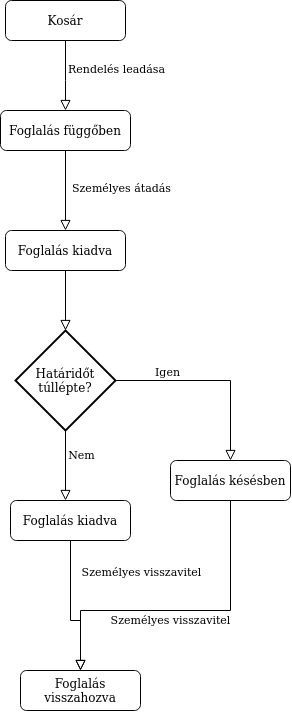
\includegraphics[width=50mm, keepaspectratio]{figures/order-flowchart.png}
  \caption{Rendelés leadásának menete}
  \label{fig:OrderChart}
\end{figure}

Egy foglalás leadása esetén a könyvből elérhető darabszámot is frissíteni kell. Ez több tábla szimultán módosításával jár,
viszont az inkonzisztencia elkerülése érdekében ennek teljesítenie kell az ACID elveket.

Mivel a Prisma jelenleg nem támogatja ilyen komplex módosítások egy utasításban történő végrehajtását, annak Transaction API
funkcióját használtam. Ennek segítségével több, egymástól független adatbázismódosítást lehet egyetlen tranzakcióba csomagolni,
így vagy minden kívánt módosítás érvényesül, vagy egyik sem.

\begin{lstlisting}[caption=Transaction API használata kölcsönzés létrehozásakor]
const createOrder = db.order.create({
  data: {
    returnDate,
    user: {
      connect: { id: userId },
    },
    books: {
      create: books.map(it => ({
        quantity: it.quantity,
        books: {
          connect: { id: it.id },
        }
      })),
    }
  },
})

const bookUpdates = books.map(book => {
  const bookUpdate = db.book.update({
    where: { id: book.id },
    data: {
      stockCount: { decrement: book.quantity }
    }
  })
  return bookUpdate
})

const [order] = await db.$transaction([createOrder, ...bookUpdates])
\end{lstlisting}

A fenti kódrészlet három fő utasításra bontható: létrehozza az \lstinline|Order| táblában az új bejegyzést a foglalásra,
beszúrja az \lstinline|Order| és \lstinline|Book| táblák közti kapcsolatot megteremtő kapcsolótáblába a megfelelő rekordokat,
valamint frissíti a \lstinline|Book| táblában lévő könyvek elérhető darabszámát.

\subsection{Kosár}

A könyv részletes nézetében lehetőség van a kosárba helyezésre. Ennek a tartalmát a felső navigációs sávon lévő bevásárlókosár
ikonra kattintva lehet megtekinteni.

\begin{figure}[!ht]
  \centering
  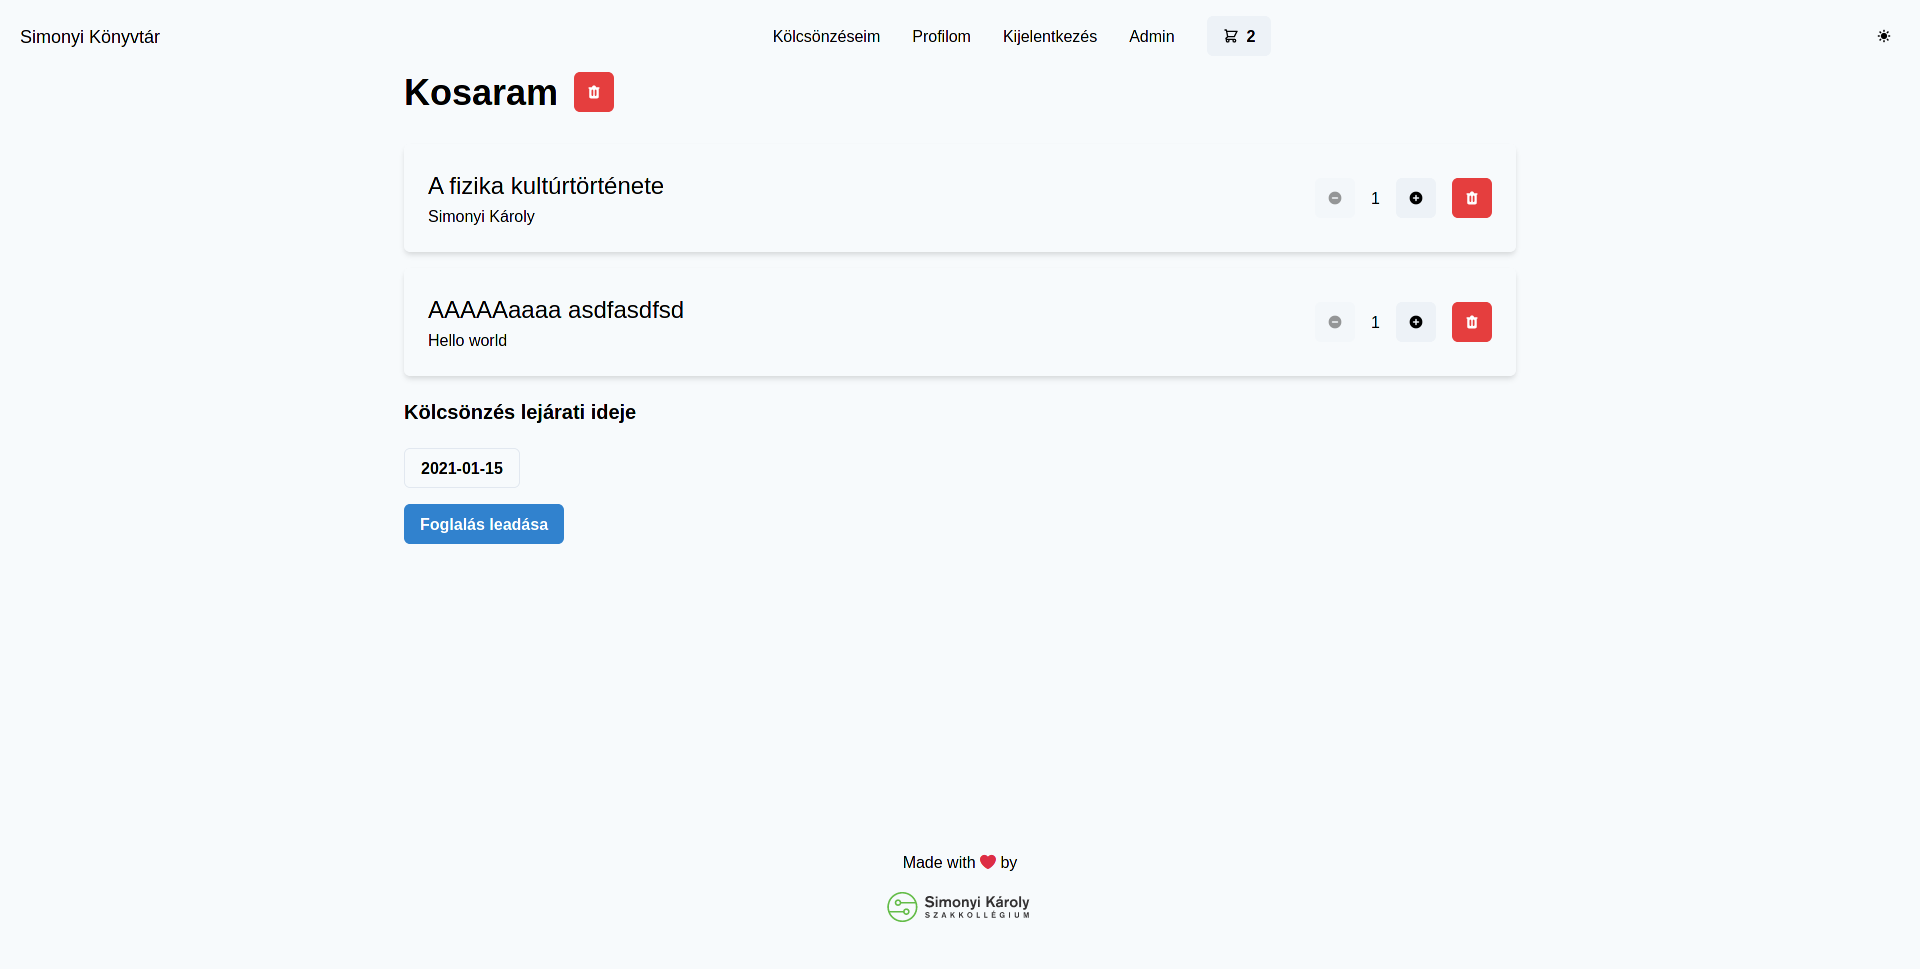
\includegraphics[width=150mm, keepaspectratio]{figures/cart.png}
  \caption{Kosár oldal}
  \label{fig:CartPage}
\end{figure}

Itt lehetőség van az egyes könyvek darabszámának állítására, illetve a kosár tartalmának módosítására.

Ezután a felhasználó ki tudja választani, hogy meddig szeretné kiválasztani a könyveket, majd a ``Foglalás leadása'' gombra kattintva
véglegesítheti azt.

A kosár adatainak tárolására a böngésző Local Storage funkcióját használtam.

Ezen megoldás előnye, hogy bejelentkezés nélkül is hozzáadhatóak könyvek és egyszerűbbé teszi az adatbázisstruktúrát.
Hátránya azonban, hogy nem kezeli a különböző böngészők (pl. asztali és mobil kliens) közötti szinkronizációt. Mivel ez utóbbi a
követelmények kidolgozása közben nem merült fel, így az egyszerűbb megoldás alkalmazása mellett döntöttem.

A kosár React-ban történő eléréséhez a \lstinline|use-persisted-state| könyvtárat vettem igénybe.

Segítségével több böngészőablakon keresztül is szinkronban tartható a kosárba helyezett könyvek,
valamint könyv hozzáadásakor illetve törlésekor automatikusan frissül minden megjelenített, kosárhoz kapcsolódó tartalom.

\subsection{Foglalás kezelése}

A foglalás leadás után a ``Kölcsönzéseim'' linkre kattintva tudjuk listázni azokat. Itt egy adott kölcsönzésre kattintva
léphetünk a részletes nézetre, ahol megjegyzéseket tudunk fűzni hozzá. Ez a funkció szolgál az átvételi időpont egyeztetésére,
problémák és egyéb igények megbeszélésére.

\begin{figure}[!ht]
  \centering
  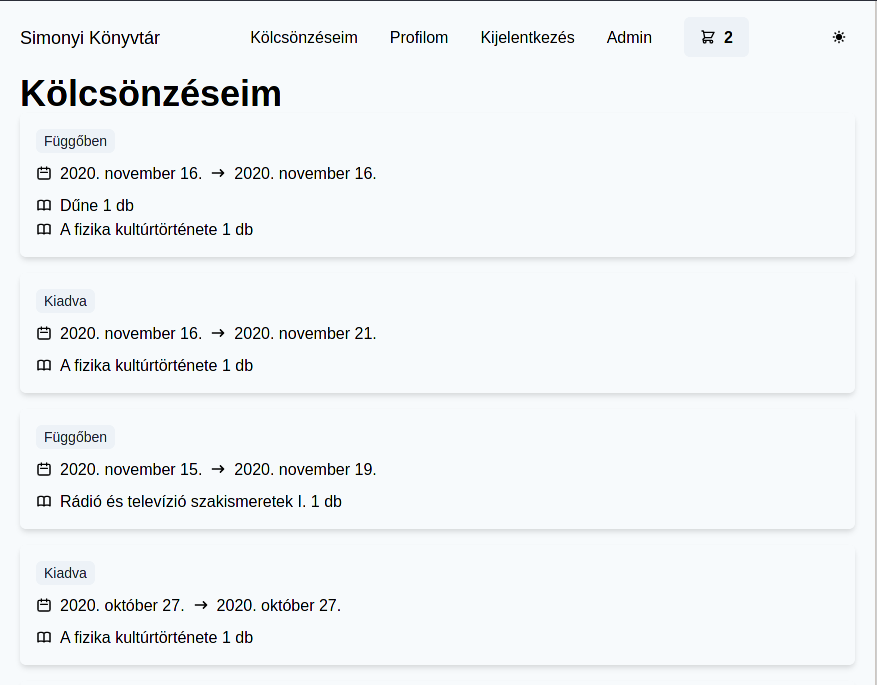
\includegraphics[width=150mm, keepaspectratio]{figures/orders-list.png}
  \caption{Kölcsönzések listázása}
  \label{fig:OrderList}
\end{figure}


\begin{figure}[!ht]
  \centering
  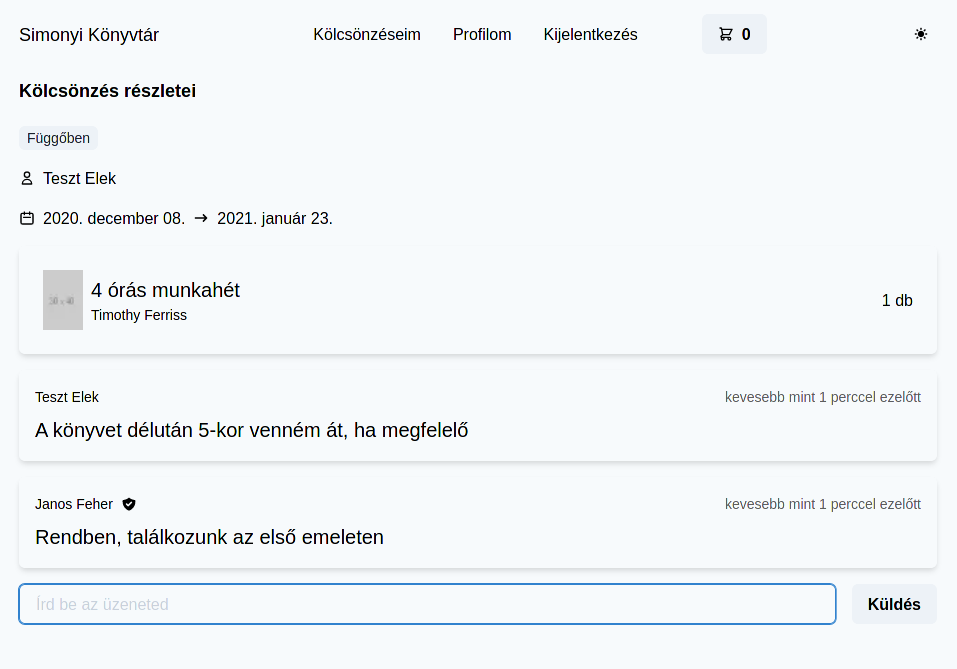
\includegraphics[width=150mm, keepaspectratio]{figures/order-detail.png}
  \caption{Kölcsönzés részletei kommentekkel}
  \label{fig:OrderDetail}
\end{figure}


\section{Admin funkciók}

Az \lstinline|ADMIN| illetve \lstinline|EDITOR| jogosultsággal rendelkező felhasználóknak lehetőségük van a rendszerben
lévő adatokat a webes felületről szerkeszteni. Ehhez a \lstinline|pages/admin| mappában külön oldalakat hoztam létre,
a backenden pedig a védett middleware-ekben valósítottam meg a funkciókat.

\subsection{Könyvek kezelése}

A könyveket egy listanézet foglalja össze. Itt lehetőség van az egyes elemek törlésére és szerkesztésére, valamint új
könyv hozzáadására. A szerkesztéshez és létrehozáshoz ugyanazt a komponenst használtam a kódduplikáció elkerülése érdekében.

\begin{figure}[!ht]
  \centering
  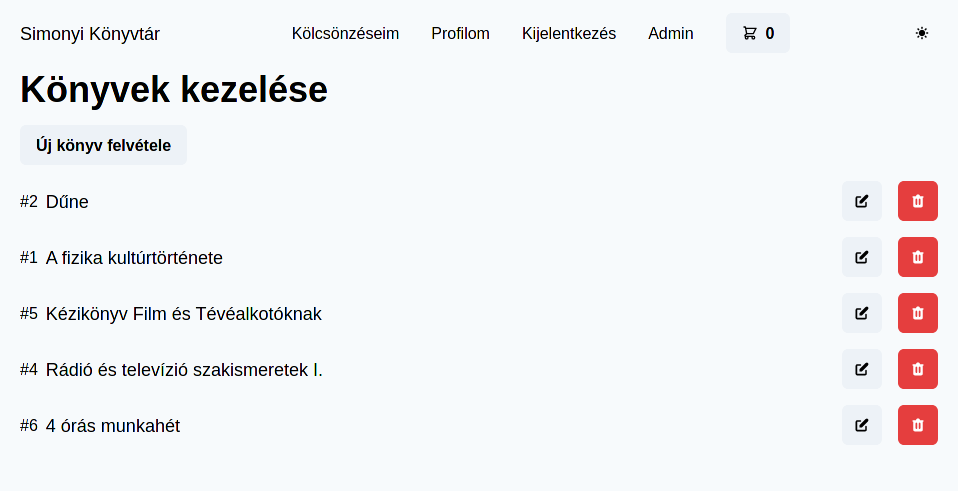
\includegraphics[width=100mm, keepaspectratio]{figures/book-admin-list.png}
  \caption{Könyvek listája az admin panelen}
  \label{fig:BookAdminList}
\end{figure}

\begin{figure}[!ht]
  \centering
  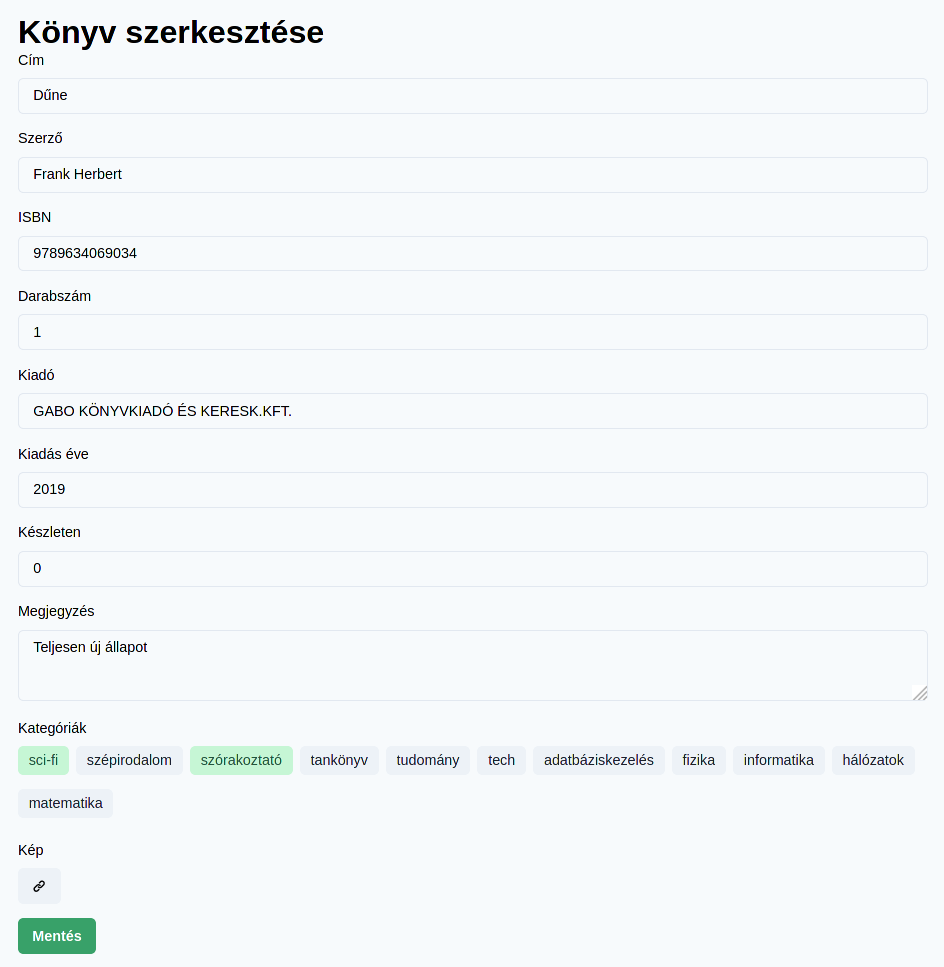
\includegraphics[width=100mm, keepaspectratio]{figures/book-edit.png}
  \caption{Könyv adatainak szerkesztése}
  \label{fig:BookEdit}
\end{figure}


\subsubsection{Fájlfeltöltés}

A könyvekhez opcionálisan megadható egy borítókép, amit a felhasználó a saját gépéről választhat ki.

Ennek a tárolására az Amazon S3 szolgáltatását választottam. A csatolt képet a frontend először elküldi a backendnek,
majd az az \lstinline|aws-sdk| könyvtárat használva feltölti a képet az S3 bucket-be, az adatbázisba csak a képet
azonosító generált kerül be. Így lehetőségünk van a képek egyszerű és adatbázisfüggetlen kezelésére.

\begin{figure}[!ht]
  \centering
  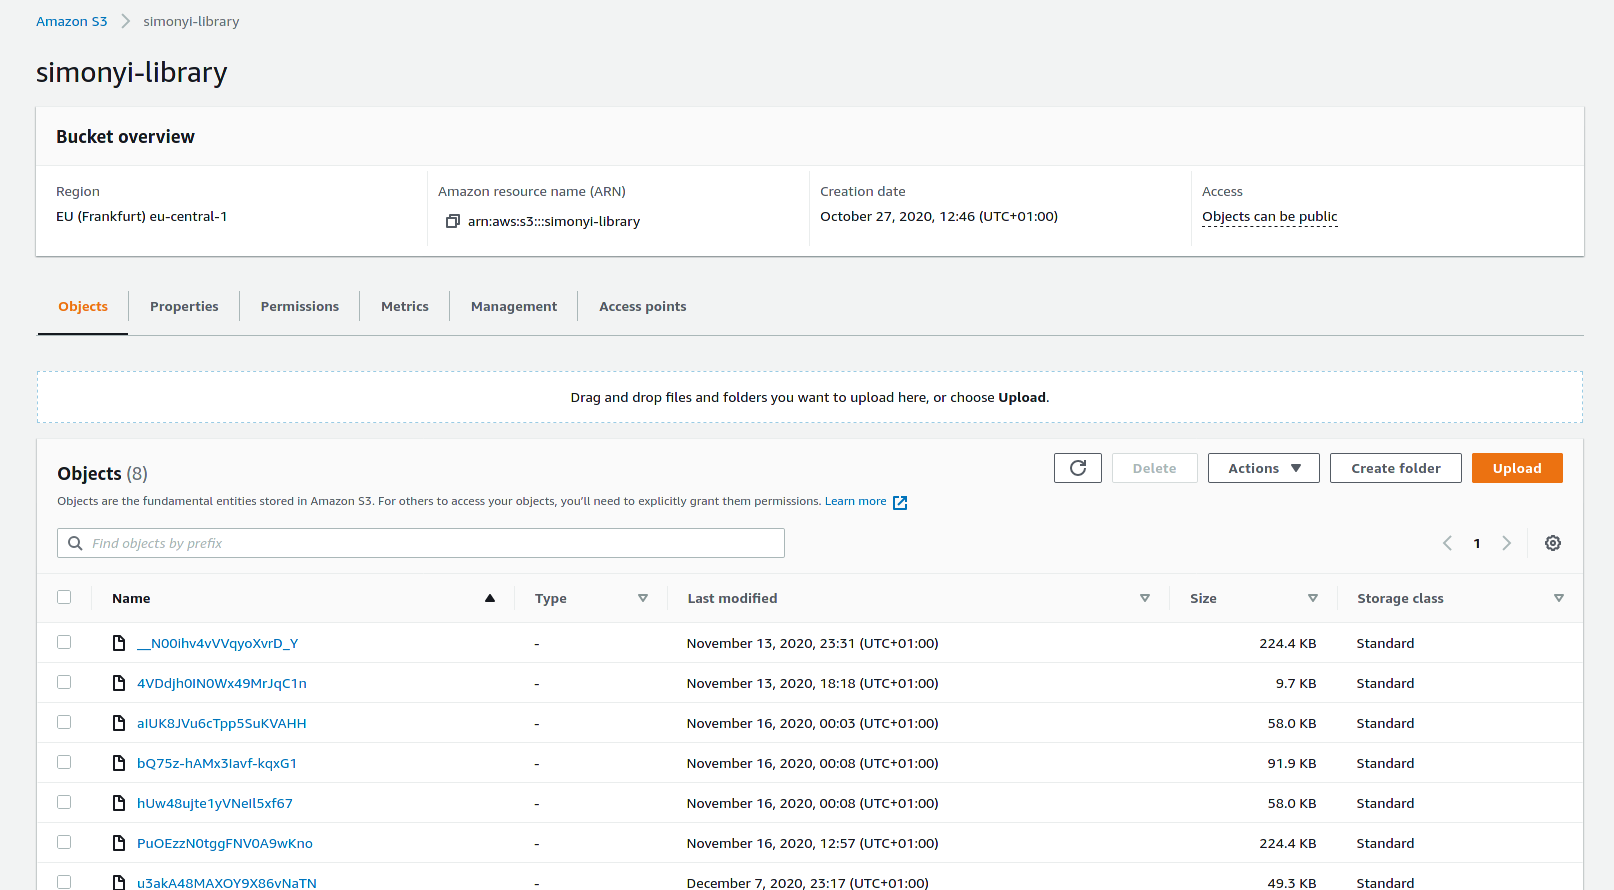
\includegraphics[width=125mm, keepaspectratio]{figures/s3-dashboard.png}
  \caption{Amazon S3 konzol}
  \label{fig:S3Console}
\end{figure}

\subsection{Kategóriák kezelése}

A kategóriákat egy összefoglaló oldalon lehet szerkeszteni és törölni. Egy elem eltávolítása esetén
minden hozzá kapcsolódó könyből is törlődik az adott kategória. Szerkesztés esetén egy felugró párbeszédablakban lehet
megadni az új nevet.

\begin{figure}[!ht]
  \centering
  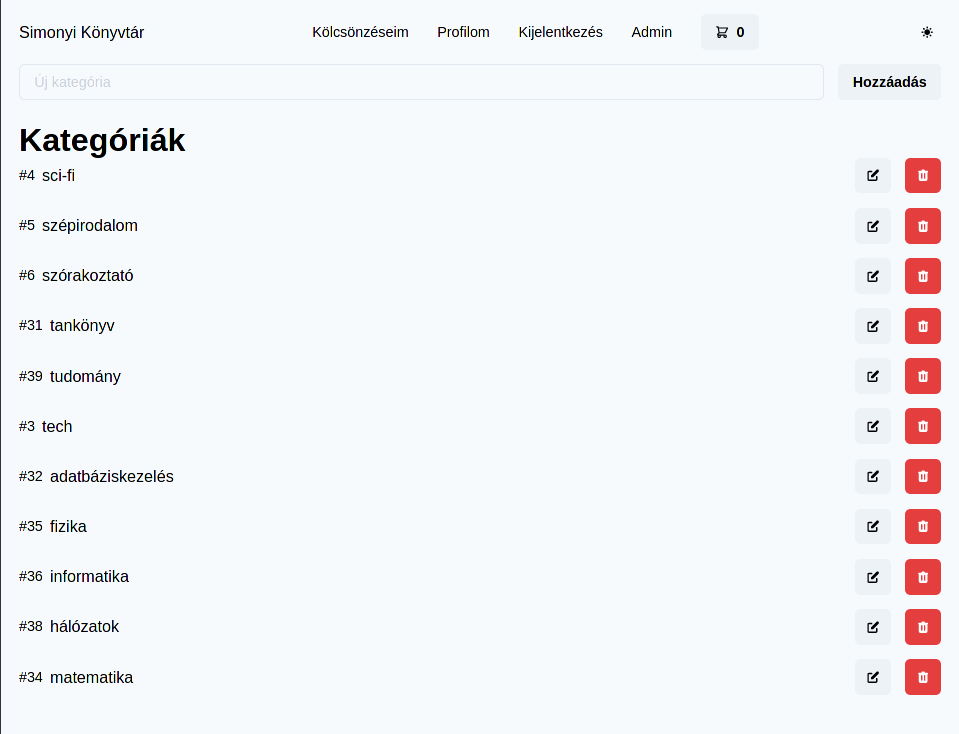
\includegraphics[width=150mm, keepaspectratio]{figures/category-admin-list.png}
  \caption{Kategóriák kezelése oldal}
  \label{fig:CategoryAdmin}
\end{figure}

\subsection{Foglalások kezelése}

% TODO
A foglalásokat egy központi oldalon lehet listázni a fontosabb információkkal.

\begin{figure}[!ht]
  \centering
  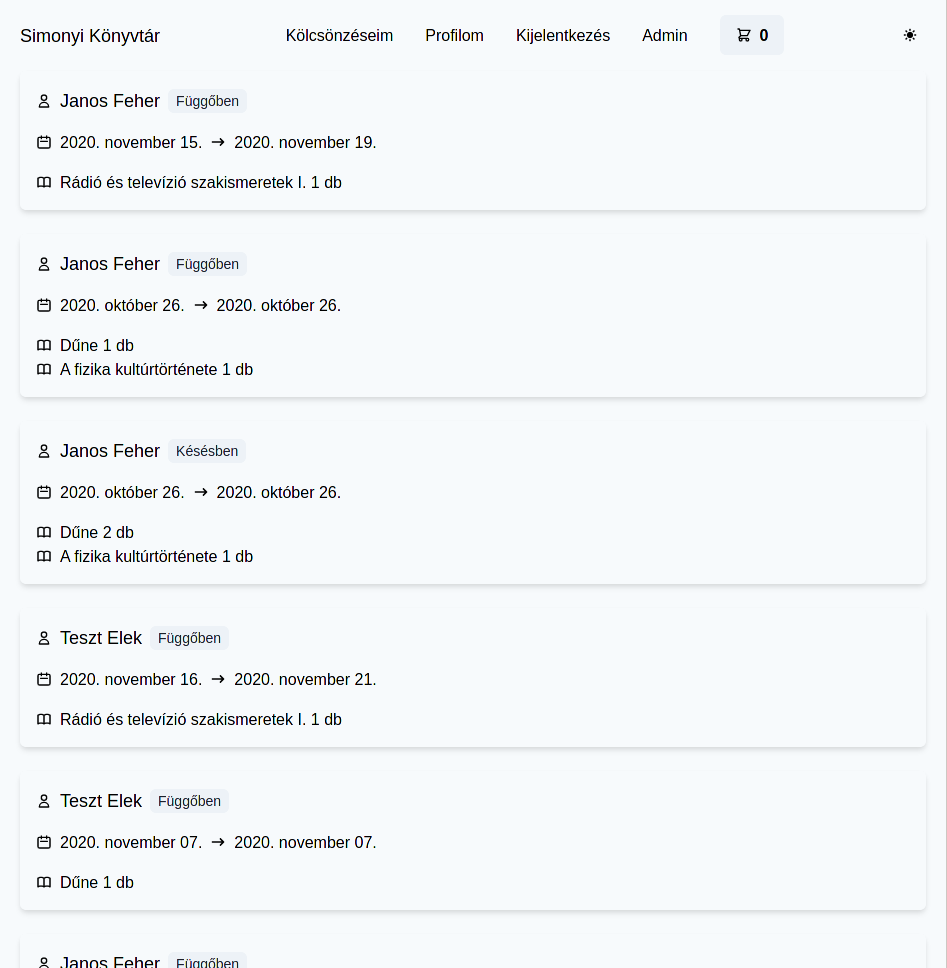
\includegraphics[width=150mm, keepaspectratio]{figures/order-admin-list.png}
  \caption{Összes foglalás listázása az adminok számára}
  \label{fig:OrderAdminList}
\end{figure}

Egy kölcsönzésre kattintva a részletes nézet jelenik meg. Itt az arra jogosultaknak lehetősége van az állapot módosítására vagy
a foglalás törlésére. Szintén itt van lehetőség minden arra jogosultnak a foglaláshoz hozzászólást fűzni.

\begin{figure}[!ht]
  \centering
  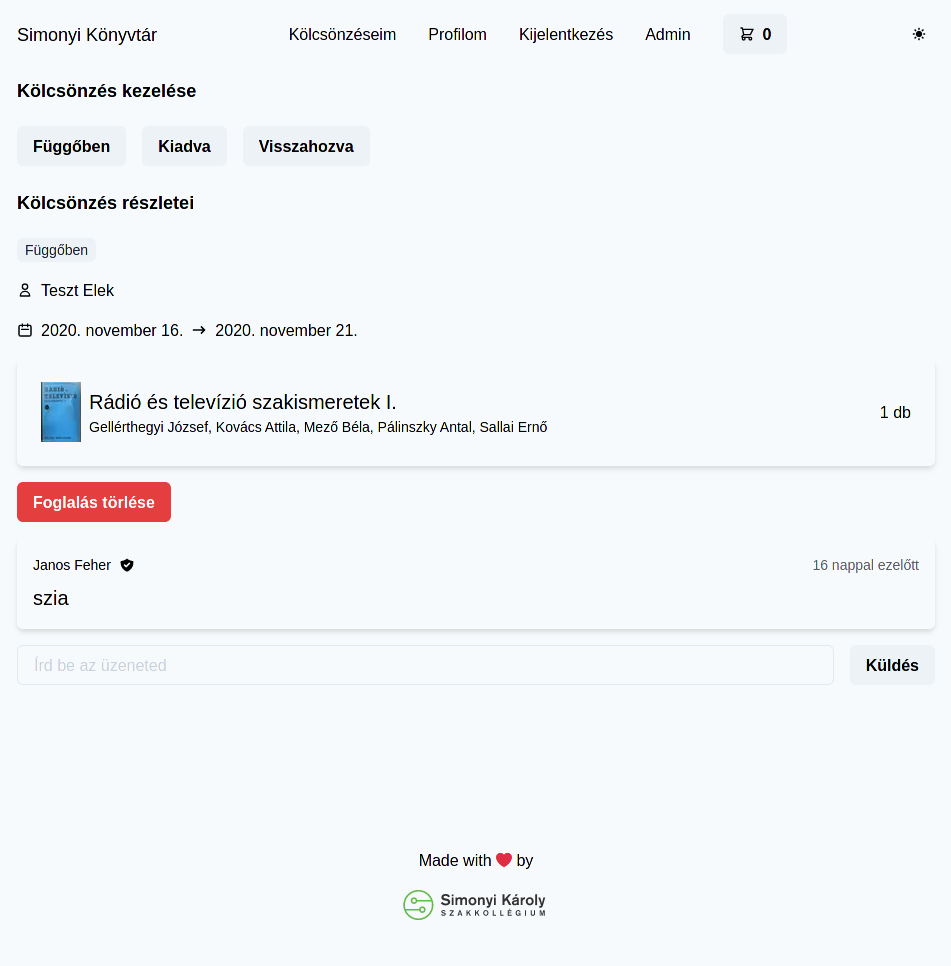
\includegraphics[width=150mm, keepaspectratio]{figures/order-admin-detail.png}
  \caption{Foglalás részletes nézete az adminok számára}
  \label{fig:OrderAdminDetail}
\end{figure}

Ha az állapot ``Visszahozva'' státuszra módosul, a foglalás leadásához hasonlóan firssülnek a könyvhöz tartozó elérhetőségi adatok.

\section{Adaptív UI}

A felület fejelsztése közben fontos volt, hogy minden oldal megfelelően működjön mobil képernyőkön is.
A Chakra UI szerencsére első kézből támogatja ezt a Responsive Styles funkciójának köszönhetően.

Ennek segítségével egy Chakra komponens tulajdonságait egy tömbben tudjuk megadni, ahol minden elem egy adott képernyőmérethez
fog társulni.

\begin{lstlisting}[caption=Chakra UI Responsive Styles használata]
<Flex direction={["column", null, "row"]}>
  <Box mr={4}>
    <NextImage
      src={
        book.image
          ? `${process.env.NEXT_PUBLIC_S3_URL}/${book.image}`
          : "https://via.placeholer.com/200x300"
      }
      width={300}
      height={450}
    />
  </Box>
  {/* Other content */}
</Flex>
\end{lstlisting}

\begin{figure}[!ht]
  \centering
  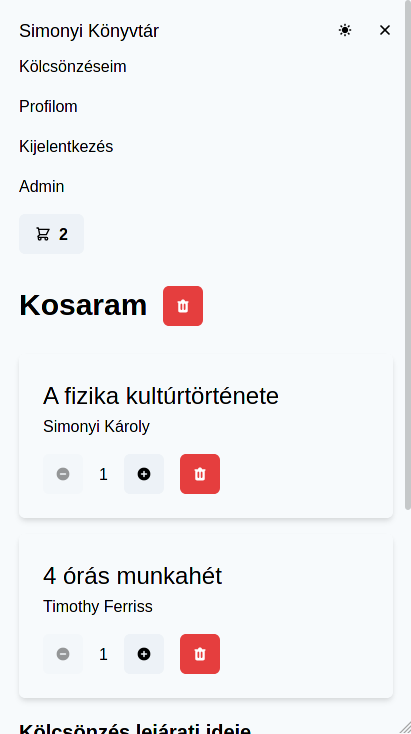
\includegraphics[width=75mm, keepaspectratio]{figures/cart-mobile.png}
  \caption{Kosár oldal mobil képernyőn, nyitott menüvel}
  \label{fig:CartMobile}
\end{figure}

\section{Dark Mode}

A Chakra UI egyik rendkívül hasznos tulajdonsága, hogy elsőrendű dark mode támogatással rendelkezik, és valamennyi komponensnek
létezik sötét módú variánsa.
Ennek segítségével gombnyomásra válthatunk a világos és sötét módok között.

\begin{figure}[!ht]
  \centering
  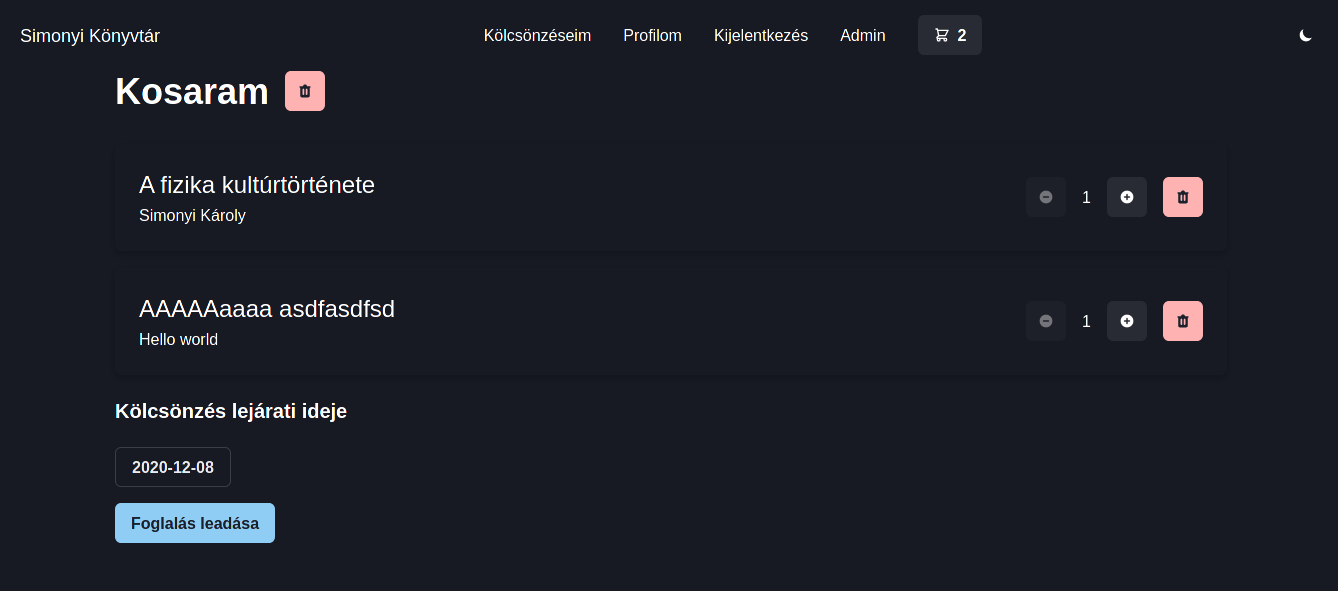
\includegraphics[width=150mm, keepaspectratio]{figures/dark-mode.png}
  \caption{Sötét téma}
  \label{fig:DarkMode}
\end{figure}

\section{Validáció}

A felhasználó által szolgáltatott adatok minden esetben potenciális veszélyforrást jelenthetnek, legyen szó XSS támadásról
vagy az adatbázis struktúrájának integritásáról. Emiatt különösen fontos a backenden történő adatok megfelelő validációja.

Ezen adatok ellenőrzésére a \lstinline|yup| könyvtárat használtam. Segítségével definiálhatunk egy sémát, ami ellen
a felhasználó által megadott adatot validálhatjuk. Ezáltal a potenciális inkonzisztenciákat még az adatbázisba írás előtt
kiszűrhetjük és tudathatjuk a felhasználóval.

\begin{lstlisting}[caption=yup validációs séma a könyvekre]
export const BookSchema = yup.object().shape({
  title: yup.string().required(),
  author: yup.string(),
  count: yup.number(),
  stockCount: yup.number(),
  isbn: yup.string(),
  publisher: yup.string(),
  publishedAt: yup.number(),
  notes: yup.string(),
  image: yup.string(),
})
\end{lstlisting}
